 %!TEX root = ../dissertation_vkslm.tex

\chapter{Neural Networks and Deep Learning} \label{ch:bg}
This chapter introduces and gives a brief overview of the theoretical concepts related to Neural Networks, and Deep Learning treated in this work. The first section gives an overview of Artificial Neural Networks, the next section we give an introduction and a general overview of the deep learning research field. Later, we
briefly describe the fundamentals of CNN's and present the Fully Convolutional Networks, which is a model concept used in this work. Finally, we present the techniques used for training our model.

\section{Neural Networks}

A biological neural network is an essential part of human brain. The human brain is a highly complex information processing system capable of interpreting large amounts of information and making decisions. It is a complex, non-linear and parallel ``computer'' consisting of millions of connected neurons \cite{haykin2009neural}. In many tasks, the human brain is more efficient than computers. For instance, the human brain can recognize a familiar face in about 100-200 ms, while modern computers require minutes or even hours for solving the same problem \cite{haykin2009neural}.

Based on examples and feedback from the ``teacher'', our brain allows us learning how to
distinguish an apple from an orange or recognize letters. Moreover, even without the ``teacher'', we
are still able to group similar patterns. Those and other strengths of human brain
challenged scientists to emulate those processes by researching how to use machines for tasks
that are common for humans. Moreover, one of the concepts that appeared as the result of that
research is the Artificial neural network (ANN) concept. Which can be thought of as an approximation or fitting function.

The first of these models was the perceptron \cite{rosenblatt1958perceptron}, which simulates a single neuron and is the elemental computing unit of an ANN. The learning rule algorithm for learning relations in data can be summarized as: for every input $x_{i}$, make a linear prediction about its label: $y^*_{i} = w^T x_{i}$
and update the weights ($w$) as,
\begin{equation}
w \leftarrow w + x_{i}(y_{i} - y^*_{i})
\end{equation}

Nonetheless, a critical evaluation by Minsky and Papert \cite{papert1969perceptrons} showed that ``for data sets that are not linearly separable, the perceptron learning algorithm will never converge'' \cite{bishop2006pattern}. This observation is related to the perceptron's limited representational power, the learning rule only converges to the correct solution if the data is linearly separable.

Stacking several perceptron units together in one layer and connecting these
stacks sequentially, without connections between the neurons in the same layer,
produces what is known as a multilayer perceptron (MLP) neural network. A MLP can be thought of as a function that maps from input to output vectors. Since the behavior of the function is parameterized by the connection weights, a single MLP is capable of instantiating many different functions. It has been proven \cite{hornik1989multilayer} that a MLP
with a single hidden layer can approximate any continuous function on a compact input domain to arbitrary precision. For this reason MLPs are said to be \textit{universal function approximators} \cite{hornik1989multilayer}.

%...
%
%Deep learning allows computational models that are composed of multiple processing layers to learn representations of
%data with multiple levels of abstraction. These methods have dramatically improved the state-of-the-art in speech rec-
%ognition, visual object recognition, object detection and many other domains such as drug discovery and genomics. Deep
%learning discovers intricate structure in large data sets by using the backpropagation algorithm to indicate how a machine
%should change its internal parameters that are used to compute the representation in each layer from the representation in
%the previous layer. Deep convolutional nets have brought about breakthroughs in processing images, video, speech and
%audio

%As redes Multi-Layer Perceptron (MLP) podem ser consideradas uma generalização do
%Perceptron. Isso se explica por este tipo de rede apresentar, além das típicas camadas de
%entrada e saída, pelo menos uma camada intermediária ou camada escondida [11].
%22A camada de entrada é onde os neurônios representam as variáveis consideradas entra-
%das do problema. A camada intermediária é a responsável pela solução de problemas não
%lineares, uma das principais características deste tipo de rede e que a difere do Perceptron
%e Adaline. Por causa disso, problemas do mundo real, que são considerados funções linear-
%mente não separáveis, podem ser resolvidos através de uma rede MLP. Os neurônios desta
%camada possuem geralmente uma função de ativação sigmoidal que pode ser a logística
%ou a tangente hiperbólica [13].
%A camada de saída representa a resposta da rede e é onde se encontra a variável
%desejada. Em geral, essa variável é aquela que se deseja prever ou classicar. Os neurônios
%desta camada, além da função de ativação sigmoidal, também podem apresentar uma
%função do tipo linear.

\begin{figure}[!htb]
\centering
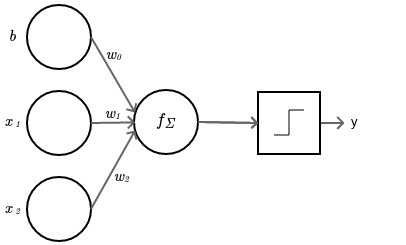
\includegraphics[width=3.4in]{perceptron}
\caption{Perceptron representation. $x_{1}$ and $x_{2}$ represent the input signal, $w_{1}$ and $w_{2}$ the weights, $f_{\sum}$ is the activation function (in this case, a step function) and the output signal is given by $y$.}
\label{perceptron}
\end{figure}

\begin{figure}[!htb]
\centering
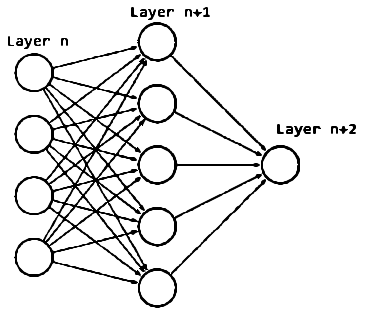
\includegraphics[width=4.5in]{mlp}
\caption{Multilayer perceptron representation. Each layer contains several perceptron units, which are then connected to units in the subsequent layer.}
\label{mlp}
\end{figure}

\begin{figure}[!htb]
\centering
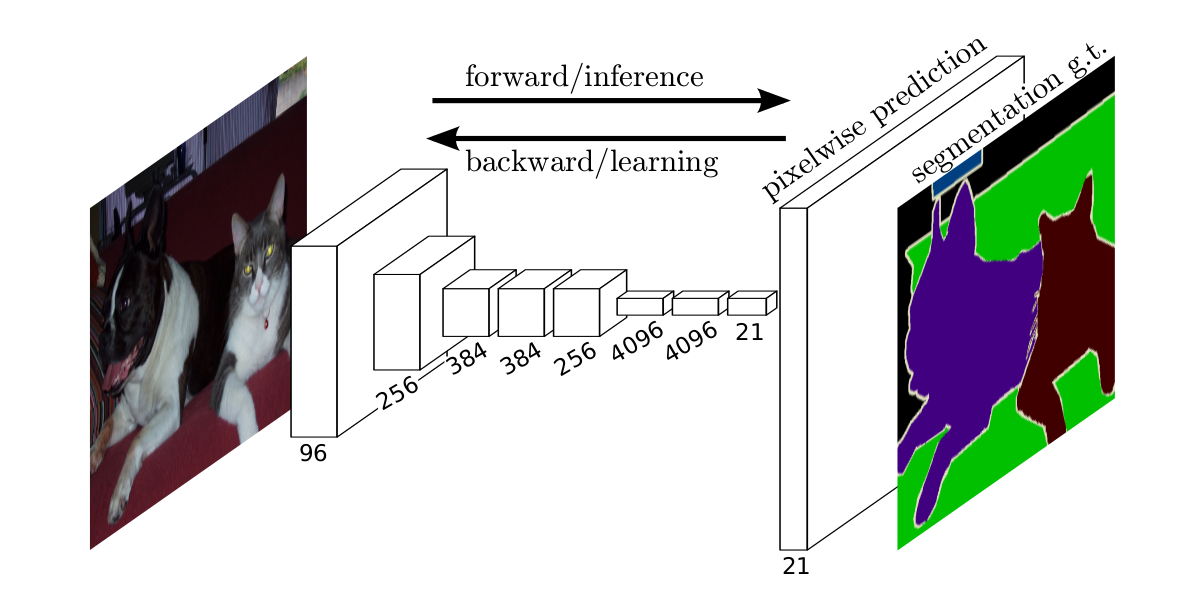
\includegraphics[width=6.5in]{fcn-arch}
\caption{Fully convolutional networks can efficiently learn to make dense predictions for
per-pixel tasks like semantic segmentation. Extracted from \cite{long2015fully}}
\label{fcn-arch}
\end{figure}

\begin{figure}[!htpb]
\centering
 \subfloat[Sigmoid]{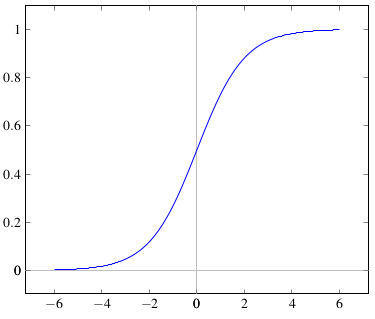
\includegraphics[width=2.5in]{sigmoid}} 
\hspace*{0.2in} % separation between the subfigures
\subfloat[Tanh] {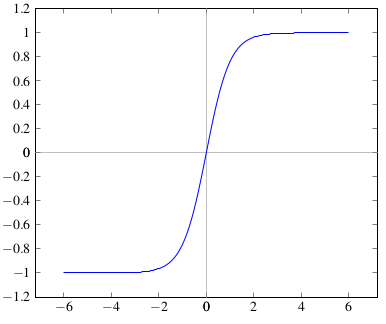
\includegraphics[width=2.5in]{tanh}}
\\
\subfloat[ReLU] {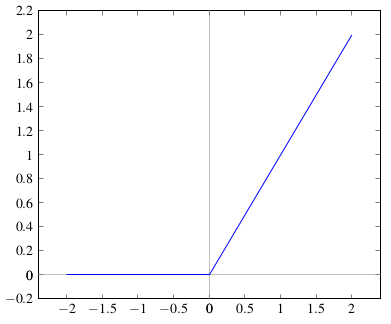
\includegraphics[width=2.5in]{relu}}
\hspace*{0.2in} % separation between the subfigures
\subfloat[LReLU] {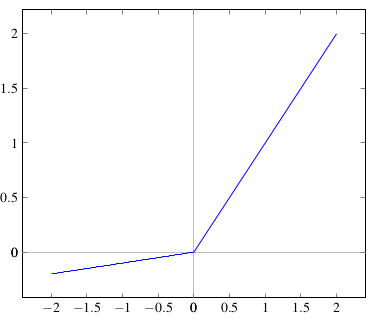
\includegraphics[width=2.5in]{lrelu}}


\caption{Neural network activation functions. } \label{fig:activation}
\end{figure}

\begin{figure}[!htb]
\centering
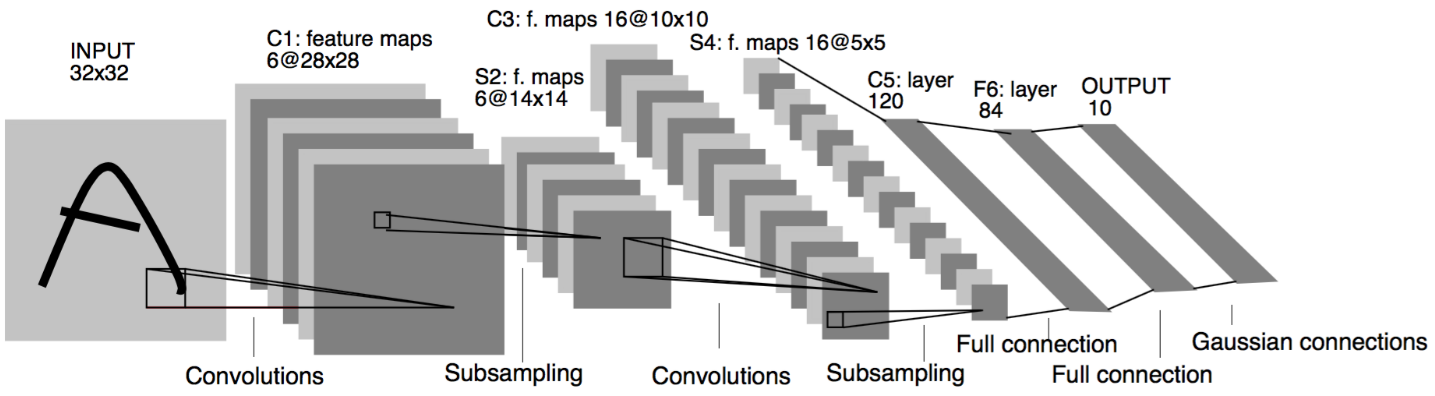
\includegraphics[width=5.5in]{lenet}
\caption{Lenet, \cite{lecun1998gradient}.}
\label{lenet}
\end{figure}

\begin{figure}[!htb]
\centering
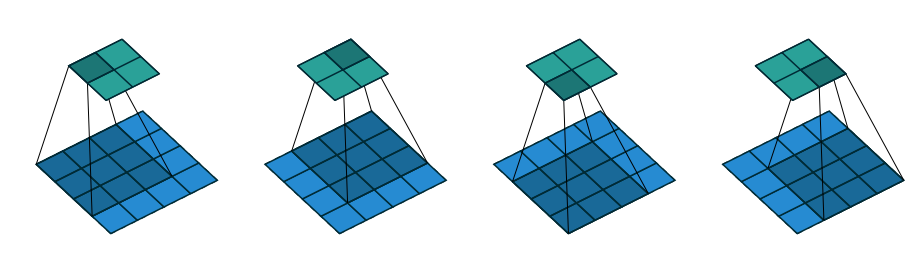
\includegraphics[width=5.5in]{conv-operation}
\caption{Convolving a 3x3 kernel over a 4x4 input. Extracted from \cite{dumoulin2016guide}. }
\label{fig:convop}
\end{figure}

\begin{figure}[!htb]
\centering
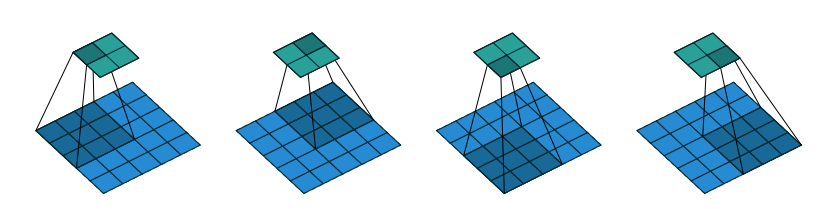
\includegraphics[width=5.5in]{conv-operation-strides}
\caption{Convolving a 3x3 kernel over a 5x5 input using 2x2 strides. Extracted from \cite{dumoulin2016guide}. }
\label{fig:convop-stride}
\end{figure}

Figure \ref{fig:convop}, Figure \ref{fig:convop-stride}. Simple convolution \footnote{Animated representation can be found in: \url{https://raw.githubusercontent.com/vdumoulin/conv_arithmetic/master/gif/no_padding_no_strides.gif}}
With strides \footnote{Animated representation of strides can be found in: \url{https://raw.githubusercontent.com/vdumoulin/conv_arithmetic/master/gif/no_padding_strides.gif}}

%ANNs can generally be thought of as an approximation or fitting function. 

% https://people.eecs.berkeley.edu/~jonlong/long_shelhamer_fcn.pdf
%Convolutional networks are driving advances in recognition.
%Convnets are not only improving for whole-image
%classification [22, 34, 35], but also making progress on local
%tasks with structured output. These include advances
%in bounding box object detection [32, 12, 19], part and keypoint
%prediction [42, 26], and local correspondence [26, 10].

\subsection{Backpropagation}


%feedforward get the output error after the signal propagation
%
%backpropagation uses the output layer error to adjust the weights


\subsection{Loss function}
\subsection{Activation function}
\subsubsection{Linear}
\subsubsection{Sigmoid}
\subsubsection{ReLU}
\subsubsection{LReLU}
\section{Convolutional Neural Networks}
\subsection{Layers}
\subsubsection{Convolution}
\subsubsection{Transposed Convolution}
\lipsum[1-1]
%https://arxiv.org/pdf/1603.07285.pdf p 19
%The need for transposed convolutions generally arises from the desire to use a
%transformation going in the opposite direction of a normal convolution, i.e., from
%something that has the shape of the output of some convolution to something
%that has the shape of its input while maintaining a connectivity pattern that
%is compatible with said convolution. For instance, one might use such a transformation
%as the decoding layer of a Convolutional Autoencoder or to project
%feature maps to a higher-dimensional space.

\section{Neural Networks training}
\lipsum[1-1]
\subsection{Weight initialization}
\subsubsection{Uniform}
\subsubsection{Glorot} 
\subsection{Optimization algorithm}
\subsubsection{Stochastic Gradient Descent}
\subsubsection{Adaptive Moment Estimation}